\documentclass[t]{beamer}
\mode<presentation>

\usepackage{etex}

\usetheme{Madrid}
% other themes: Warsaw, AnnArbor, Antibes, Bergen, Berkeley, Berlin, Boadilla, boxes, CambridgeUS, Copenhagen, Darmstadt, default, Dresden, Frankfurt, Goettingen,
% Hannover, Ilmenau, JuanLesPins, Luebeck, Madrid, Maloe, Marburg, Montpellier, PaloAlto, Pittsburg, Rochester, Singapore, Szeged, classic

\setbeamertemplate{navigation symbols}{\insertslidenavigationsymbol}

\usecolortheme{dolphin}
%\usecolortheme{seagull}
% color themes: albatross, beaver, beetle, crane, default, dolphin, dov, fly, lily, orchid, rose, seagull, seahorse, sidebartab, structure, whale, wolverine

%\usefonttheme{serif}
% font themes: default, professionalfonts, serif, structurebold, structureitalicserif, structuresmallcapsserif

% pdf is displayed in full screen mode automatically
%\hypersetup{pdfpagemode=FullScreen}

%\AtBeginSection[]
%{
%  \begin{frame}<beamer>
%    \frametitle{Outline}
%    \tableofcontents[currentsection,currentsubsection]
%  \end{frame}
%}

% define your own colours:
\definecolor{Red}{rgb}{1,0,0}
\definecolor{Blue}{rgb}{0,0,1}
\definecolor{Green}{rgb}{0,1,0}
\definecolor{magenta}{rgb}{1,0,.6}
\definecolor{lightblue}{rgb}{0,.8,1}
\definecolor{lightpurple}{rgb}{.6,.4,1}
\definecolor{gold}{rgb}{.6,.5,0}
\definecolor{orange}{rgb}{1,0.4,0}
\definecolor{hotpink}{rgb}{1,0,0.5}
\definecolor{newcolor2}{rgb}{.5,.3,.5}
\definecolor{newcolor}{rgb}{0,.3,1}
\definecolor{newcolor3}{rgb}{1,0,.35}
\definecolor{darkgreen1}{rgb}{0, .35, 0}
\definecolor{darkgreen}{rgb}{0, .6, 0}
\definecolor{darkred}{rgb}{.75,0,0}

\xdefinecolor{olive}{cmyk}{0.64,0,0.95,0.4}
\xdefinecolor{purpleish}{cmyk}{0.75,0.75,0,0}

%\usepackage{beamerinnerthemerounded}
% inner themes include circles, default, inmargin, rectangles, rounded

%\usepackage{beamerouterthemesmoothbars}
% outer themes include default, infolines, miniframes, shadow, sidebar, smoothbars, smoothtree, split, tree

\useoutertheme[subsection=false]{smoothbars}

% to have the same footer on all slides
\setbeamertemplate{footline}[text line]{
\raisebox{3pt}{
\includegraphics[height=15pt]{su-long.eps}}\hfill 
\raisebox{5pt}{Math 207:  Statistics}\hfill 
\raisebox{5pt}{The Average and the Standard Deviation}\hfill
\raisebox{5pt}{\insertframenumber/\pageref{lastpage}}}
%\setbeamertemplate{footline}[text line]{} % or empty footer

% include packages
\usepackage{subfigure}
\usepackage{multicol}
\usepackage{amsmath}
\usepackage{epsfig}
\usepackage{graphicx}
\usepackage[all,knot]{xy}
\xyoption{arc}
\usepackage{url}
\usepackage{multimedia}
\usepackage{hyperref}
\usepackage{setspace}

\title{Math 207:  Statistics}
\subtitle{The Average and the Standard Deviation}
\author{Ralph Wojtowicz}
\institute{Mathematics Department\\ Shenandoah University}
%\date{\scriptsize 20 January 2012}

\usepackage{pstricks,pst-grad,pst-text,pst-node,multido,pst-plot,calc,pst-3dplot}

\begin{document}

%\frame[plain]{
%	\titlepage
%}


\begin{frame}[plain]
\definecolor{myblue}{rgb}{0,0,0.6}
\definecolor{grayA}{rgb}{0.95,0.95,0.95}
\definecolor{grayB}{rgb}{0.98,0.98,0.98}
\begin{center}
%\begin{pspicture}(0,0)(7,4.8)
\begin{pspicture}(-6,-7)(6,2)
\rput(0,-1.7){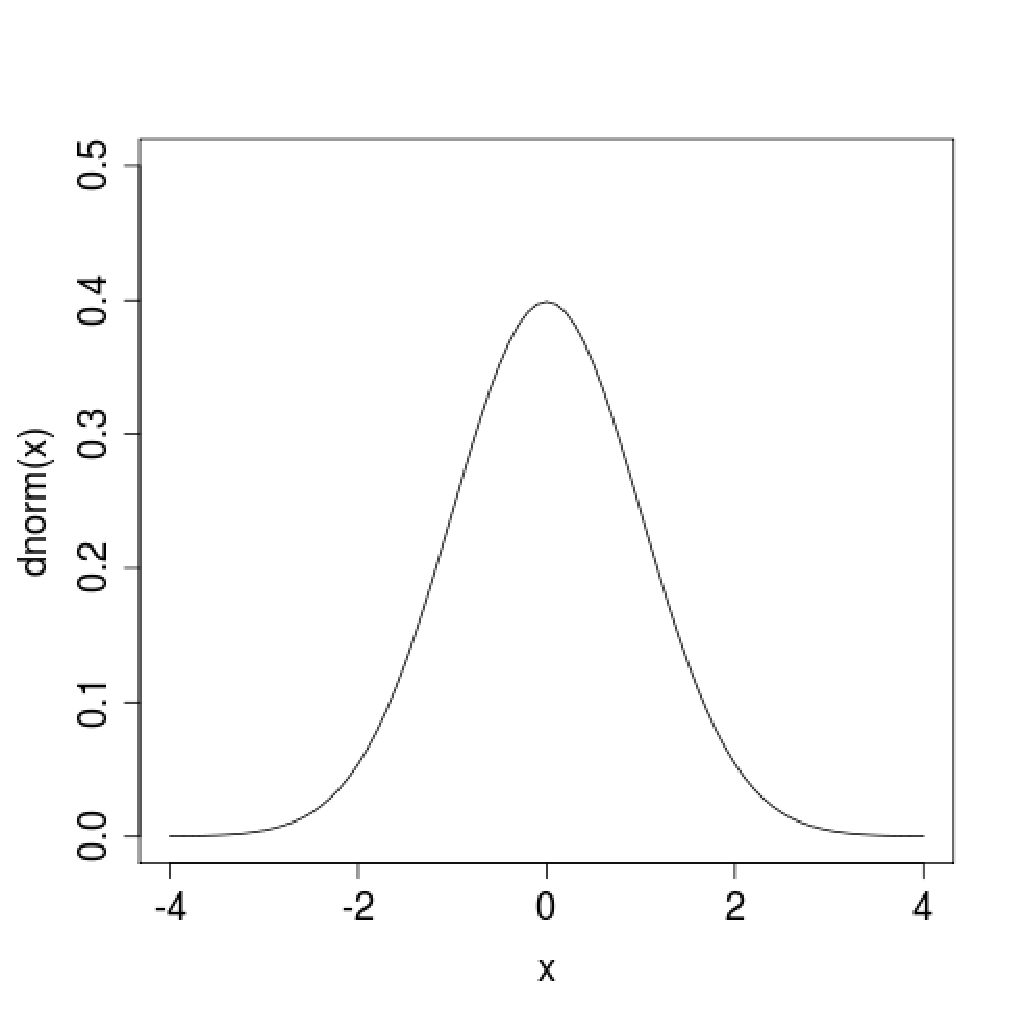
\includegraphics[height=1.8in]{../dnorm.eps}}
\psframe[linewidth=0.02,linecolor=gray](-6.2,-7)(6.2,2.2)
\psframe[linewidth=0.02,linecolor=gray](-6.15,-6.95)(6.15,2.15)
\rput(0,1.4){\color{myblue}\large Math 207:  Statistics}
\rput(0,0.6){\color{myblue}The Average and the  Standard Deviation}
%\psframebox(0,0)(4,4)
\rput(0,-4.2){\scriptsize Dr.~Ralph Wojtowicz}
\rput(0,-4.7){\scriptsize Mathematics Department}
\rput(0,-5.5){
\includegraphics[height=1cm]{su-long.eps}}
%
%\rput(0,-6.5){\scriptsize 20 January 2012}
\end{pspicture}
\end{center}


\end{frame}


\addtocounter{page}{-1}
\addtocounter{framenumber}{-1}

{\footnotesize
\frame{\tableofcontents}
}

\section{Introduction}
\subsection{Introduction}
\begin{frame}[t]\frametitle{Introduction}
{\small
\begin{itemize}
\item We have studied tools such as histograms for summarizing and gaining insights into data.
\item The \textbf{center} (average or mean and median) and \textbf{spread} 
  (standard deviation or sd) are numerical tools
  of descriptive statistics.
\item Range ($\mbox{maximum value} - \mbox{minimum value}$), interquartile range, and quantiles are 
  other descriptive statistics we will meet.
\end{itemize}
\begin{center}
{\footnotesize\begin{pspicture}(0,0)(3,4.2)
\psset{linewidth=0.02}
\rput(1.5,4){\rnode{Statistics}{\psframebox{Statistics}}}
\pnode(1.5,3){NULL}
\rput(0,3){\ovalnode{Descriptive}{\hspace{-8pt}\tiny\color{blue}
    \begin{tabular}{c}Descriptive\\ Statistics\end{tabular}\hspace{-8pt}}}
\rput(3,3){\ovalnode{Inferential}{\hspace{-8pt}\tiny\begin{tabular}{c}Inferential\\ Statistics\end{tabular}\hspace{-8pt}}}
\rput[t](0,2){\tiny\rnode{ID}{\psframebox{\hspace{-4pt}\begin{tabular}{l}Includes\\ 
        $\bullet$ Collecting\\ 
        $\bullet$ Organizing\\ 
        $\bullet$ \color{blue}Summarizing\\ 
        $\bullet$ Presenting\\ 
        {\color{blue}data}\end{tabular}\hspace{-4pt}}}}
\rput[t](3,2){\tiny\rnode{II}{\psframebox{\hspace{-4pt}\begin{tabular}{l}Includes\\ 
        $\bullet$ Making inferences\\ 
        $\bullet$ Hypothesis testing\\ 
        $\bullet$ Determining \\ \hphantom{$\bullet$} relationships\\ 
        $\bullet$ Making predictions\\ \end{tabular}\hspace{-4pt}}}}
\ncline{->}{Statistics}{NULL}
\ncline{->}{NULL}{Descriptive}
\ncline{->}{NULL}{Inferential}
\ncline{->}{Descriptive}{ID}
\ncline{->}{Inferential}{II}
\end{pspicture}}
\end{center}
}
\end{frame}

%\subsection{Levels of Detail}
%\begin{frame}[t]\frametitle{Levels of Detail}
%
%\end{frame}

\section[Average]{The Average}
\subsection[Average]{The Average (Mean)}
\begin{frame}[t]\frametitle{The Average (Mean)}
{\small
\begin{itemize}
\item The \textbf{average} (\textbf{mean}) of a list of numbers equals their sum, divided by how many there are.\vspace{-10pt}
\[\mbox{average (mean) of a list of numbers} = \frac{x_1+x_2+\cdots + x_n}{n}=\frac{1}{n}\,\sum_{i=1}^n\,x_i\vspace{-8pt}\]
\item Example:  The list $9$, $1$, $2$, $2$, $0$ has $n=5$ entries.  Its average is
\[\frac{9+1+2+2+0}{5}=\frac{14}{5}=2.8\vspace{-4pt}\]
\item The histogram \textit{balances} when supported at the average.
\end{itemize}
{\footnotesize
   \begin{center}
   \begin{pspicture}(0,-0.2)(9,0.8)
   \psset{yunit=0.95}
   \psframe[fillstyle=solid,fillcolor=lightblue](-0.5,0)(0.5,0.5)
   \psframe[fillstyle=solid,fillcolor=lightblue](0.5,0)(1.5,0.5)
   \psframe[fillstyle=solid,fillcolor=lightblue](1.5,0)(2.5,1)
   \psframe[fillstyle=solid,fillcolor=lightblue](8.5,0)(9.5,0.5)
   \psline(0,0)(10,0)
   \rput[t](0,-0.1){0}\rput[t](1,-0.1){1}\rput[t](2,-0.1){2}\rput[t](3,-0.1){3}\rput[t](4,-0.1){4}
   \rput[t](5,-0.1){5}\rput[t](6,-0.1){6}\rput[t](7,-0.1){7}\rput[t](8,-0.1){8}\rput[t](9,-0.1){9}
   \psline[linewidth=0.05]{->}(2.8,-0.6)(2.8,0)
   \end{pspicture}
   \end{center}}
\begin{itemize}
\item In R we can compute the mean of a list of numbers as follows:\\
  \texttt{> x <- c(9, 1, 2, 2, 0)}\\
  \texttt{> mean(x)}\\
  \texttt{[1] 2.8}
\end{itemize}}
\end{frame}

%\subsection{Cross-Sectional and Longitudinal Surveys}
%\begin{frame}[t]\frametitle{Cross-Sectional and Longitudinal Surveys}
%
%\end{frame}


\section{Histograms}
\subsection[Histograms]{The Average and the Histogram}
\begin{frame}[t]\frametitle{The Average and the Histogram}

{\small
\begin{itemize}
\item The histogram balances when supported at the mean.
\item The first histogram below is \textbf{symmetric} about its mean.  Half the data is to the left of the mean and half
  is to the right. %In the other cases, only $1/4$ of the data is to the right.
\end{itemize}}

{\footnotesize
   \begin{center}
   \begin{pspicture}(0,-1)(9,1)
   \psset{yunit=0.95}
%   \psframe[fillstyle=solid,fillcolor=lightblue](-0.5,0)(0.5,0.5)
   \psframe[fillstyle=solid,fillcolor=lightblue](0.5,0)(1.5,0.5)
   \psframe[fillstyle=solid,fillcolor=lightblue](1.5,0)(2.5,1)
   \psframe[fillstyle=solid,fillcolor=red](2.5,0)(3.5,0.5)
   \psline(0,0)(8.5,0)
   \rput[t](0,-0.1){0}\rput[t](1,-0.1){1}%\rput[t](2,-0.1){2}
   \rput[t](3,-0.1){3}\rput[t](4,-0.1){4}
   \rput[t](5,-0.1){5}\rput[t](6,-0.1){6}\rput[t](7,-0.1){7}\rput[t](8,-0.1){8}%\rput[t](9,-0.1){9}
   \psline[linewidth=0.05]{->}(2,-0.6)(2,0)
   \rput[l](7.5,0.8){List $=$ $1$, $2$, $2$, $3$}
   \end{pspicture}

   \begin{pspicture}(0,-1)(9,1)
   \psset{yunit=0.95}
%   \psframe[fillstyle=solid,fillcolor=lightblue](-0.5,0)(0.5,0.5)
   \psframe[fillstyle=solid,fillcolor=lightblue](0.5,0)(1.5,0.5)
   \psframe[fillstyle=solid,fillcolor=lightblue](1.5,0)(2.5,1)
   \psframe[fillstyle=solid,fillcolor=red](4.5,0)(5.5,0.5)
   \psline(0,0)(8.5,0)
   \rput[t](0,-0.1){0}\rput[t](1,-0.1){1}\rput[t](2,-0.1){2}
   \rput[t](3,-0.1){3}\rput[t](4,-0.1){4}
   \rput[t](5,-0.1){5}\rput[t](6,-0.1){6}\rput[t](7,-0.1){7}\rput[t](8,-0.1){8}%\rput[t](9,-0.1){9}
   \psline[linewidth=0.05]{->}(2.5,-0.6)(2.5,0)
   \rput[l](7.5,0.8){List $=$ $1$, $2$, $2$, $5$}
   \end{pspicture}

   \begin{pspicture}(0,-1)(9,1)
   \psset{yunit=0.95}
%   \psframe[fillstyle=solid,fillcolor=lightblue](-0.5,0)(0.5,0.5)
   \psframe[fillstyle=solid,fillcolor=lightblue](0.5,0)(1.5,0.5)
   \psframe[fillstyle=solid,fillcolor=lightblue](1.5,0)(2.5,1)
   \psframe[fillstyle=solid,fillcolor=red](6.5,0)(7.5,0.5)
   \psline(0,0)(8.5,0)
   \rput[t](0,-0.1){0}\rput[t](1,-0.1){1}\rput[t](2,-0.1){2}
   %\rput[t](3,-0.1){3}
   \rput[t](4,-0.1){4}
   \rput[t](5,-0.1){5}\rput[t](6,-0.1){6}\rput[t](7,-0.1){7}\rput[t](8,-0.1){8}%\rput[t](9,-0.1){9}
   \psline[linewidth=0.05]{->}(3,-0.6)(3,0)
   \rput[l](7.5,0.8){List $=$ $1$, $2$, $2$, $7$}
   \end{pspicture}



   \end{center}}


\end{frame}


\section[Median]{Median}
\subsection[Median]{Median}
\begin{frame}[t]\frametitle{The Median}

{\small
\begin{itemize}
\item The \textbf{median} of a list of numbers is the value with half the area to the left and half to the right.
\item Examples:
  \begin{itemize}
  \item For the list $1$, $2$, $2$, $3$, the median is 2 (as is the mean).
  \item For the list $1$, $2$, $2$, $5$, the median is 2 (but the mean is 2.5).
  \item For the list $1$, $2$, $2$, $1000$, the median is 2 (but the mean is 251.25).
  \item For the list $1$, $2$, $3$, $8$, the median is any number (such as 2.5) that is
    greater than 2 but less than 3  (but the mean is 3.5).\\
  \texttt{> x <- c(1,2,3,8)}\\
  \texttt{> median(x)}\\
  \texttt{[1] 2.5}
  \end{itemize}
\item We typically use the median rather than the mean to describe the center 
  of a histogram with a long tail (e.g.,~incomes or home prices).
\item The \textbf{mode} of a list of numbers is the most frequent value.  We will not use the mode.
\end{itemize}}
\end{frame}

\subsection{Percentiles}
\begin{frame}
\frametitle{Quantiles and Percentiles}

\footnotesize
\begin{itemize}
%\item Suppose we have a data set $x_1$, $x_2$, $\dots$, $x_n$.
\item The \textbf{median} of the data set is also called the 
    50th \textbf{percentile} because 50\% of the data is less than or equal to it.
\item The pth percentile is a number that is greater than or equal to  p\% of the data.
\item For example, the 25th percentile is the median of the first half of the data.\\
     The 75th percentile is the median of the second half of the data.
\item To compute the median or  other percentiles, you first have to put the data in order.
\item Here is how to compute these in \texttt{R}:\\[3pt]
\texttt{> x = c(2, 3, 5, 5, 6, 10, 12, 17, 19, 19, 20)}\\[3pt]
\texttt{> summary(x)}\\
\texttt{ \  Min.  1st Qu.  Median   \ \ \  Mean \ \  3rd Qu.   \ \ Max. }\\
\texttt{ \  2.00  \ \ \ \ 5.00   \ \ 10.00 \ \  10.73 \ \ \ \ 18.00  \ \ 20.00 }\\[3pt]
\texttt{> quantile(x, probs=c(0.0, 0.25, 0.35, 0.50, 0.75, 1.00))}\\
\texttt{ \ 0\% \ \ 25\%  \ \ 35\% \ \ 50\% \ \  75\%  \ \ 100\% }\\
\texttt{   2.0  \ \  5.0  \ \ 5.5 \  10.0 \   18.0 \ \    20.0 }
\end{itemize}

\end{frame}

\section[RMS]{The Root-Mean-Square}
\subsection[RMS]{The Root-Mean-Square}
\begin{frame}[t]\frametitle{The Root-Mean-Square}

{\small
\begin{itemize}
\item The \textbf{root-mean-square} (or RMS) of a list of numbers measures the average magnitude (ignoring signs)
  of the numbers in the list.
\end{itemize}
\[\mbox{RMS size of a list of numbers} = \sqrt{\frac{x_1^2 + x_2^2 + \cdots + x_n^2}{n}} 
   = \sqrt{\frac{1}{n}\,\sum_{i=1}^n x_i^2}\]
\begin{itemize}
\item Example:   The list $0$, $5$, $-8$, $7$, $-3$ has $n=5$ entries.  Its RMS size is
\end{itemize}
{\footnotesize\[\sqrt{\frac{0^2+5^2+(-8)^2 + 7^2 + (-3)^2}{5}}=\sqrt{\frac{0+25+64+49+9}{5}}
   =\sqrt{\frac{147}{5}}=\sqrt{29.4}\approx 5.4\]}
\begin{itemize}
\item The calculation steps are:  (1)~{\color{blue}\textbf{square}} the entries of the list, 
  (2)~take the {\color{blue}\textbf{mean}} of this new list, and (3)~take
  the square {\color{blue}\textbf{root}} of this mean.
\item RMS is used to compute the sd (or spread) of a list of numbers.
\end{itemize}
}

\end{frame}


\section[SD]{The Standard Deviation}
\subsection[SD]{The Standard Deviation}
\begin{frame}[t]\frametitle{The Standard Deviation}
{\small
\begin{itemize}
\item \textbf{Standard deviation (sd)} measures the \textbf{spread} of the data.
   \begin{itemize}
   \item Roughly 68\% of the data falls within one sd of the average.
   \item Roughly 95\% of the data falls within two sds of the average.
   \end{itemize}
\item Average (mean) and median are measures of the center of the data.
\item Units of sd and average are the same as those of the data.
\item \textbf{Variance} is $\mbox{sd}^2$.
\end{itemize}


}
\end{frame}

%\section{Computing SD}
\subsection{Computing the Sample sd}
\begin{frame}[t]\frametitle{Computing the Population Standard Deviation (SD)}
{\small
\begin{itemize}
\item The \textbf{standard deviation} (\textbf{SD}) 
  of a list of numbers equals the RMS deviation from average. SD is
  \textbf{population standard deviation}.\vspace{-9pt}
\end{itemize}
{\footnotesize
\begin{align*}
\mbox{SD of a list of numbers} &= \sqrt{\frac{(x_1-\mbox{mean})^2+(x_2-\mbox{mean})^2+\cdots + (x_n-\mbox{mean})^2}{n}}\\
                               &=\sqrt{\frac{1}{n}\,\sum_{i=1}^n\,(x_i-\mbox{mean})^2}
\end{align*}}\vspace{-12pt}
\begin{itemize}
\item Example:  The list $20$, $10$, $15$, $15$ has $n=4$ entries.  
To compute the SD, we first need the mean of the list.
\end{itemize}
{\footnotesize\[\mbox{mean}=\frac{1}{4}\,(20+10+15+15) = 60/4 = 15\]}\vspace{-15pt}
\begin{itemize}
\item[] We then calculate the mean of the square deviations from this average.
\end{itemize}\vspace{2pt}
{\footnotesize
\[\frac{(20-15)^2 + (10-15)^2 + (15-15)^2 + (15-15)^2}{4}=\frac{5^2 + 5^2}{4}=\frac{50}{4}=12.5\vspace{-8pt}\]}
\begin{itemize}
\item[] We then take the square root:  $\mbox{SD}=\sqrt{12.5}\approx 3.5$.
\end{itemize}
}
\end{frame}

\section{sd}
\subsection[sd]{Computing SD and SD$+$ (sd) in R}
\begin{frame}[t]\frametitle{Computing Sample Standard Deviation (sd)}
{\small
\begin{itemize}
\item Most calculators (and statistical software such as \texttt{R}) compute
   the \textbf{sample standard deviation}:
\begin{align*}
\mbox{sd}&= \sqrt{\frac{(x_1-\mbox{mean})^2+(x_2-\mbox{mean})^2+\cdots + 
           (x_n-\mbox{mean})^2}{n-1}}\\
                               &=\sqrt{\frac{1}{n-1}\,\sum_{i=1}^n\,(x_i-\mbox{mean})^2}
\end{align*}
%\item In \texttt{R}, \texttt{sd(x)} is $\mbox{SD}^+$ of the list \texttt{x}.
\item To compute the population SD using \texttt{R}, we must correct the denominator:
\\[3pt]
      \texttt{> x <- c(20,10,15,15)}\\[3pt]
      \texttt{> sd(x)}\\
      \texttt{[1] 4.082483}\\[3pt]
 %
      \texttt{> n = length(x)}\\
      \texttt{> sd(x) * sqrt((n - 1))/n}\\
      \texttt{[1] 3.535534}\\[3pt]
\end{itemize}
}
\label{lastpage}
\end{frame}

\end{document} 
